\documentclass[tikz,border=6mm]{standalone}
\usepackage{tikz}
\usetikzlibrary{shapes.geometric,arrows.meta,positioning,fit,backgrounds,calc}
\usepackage{amsmath,amssymb}
\usepackage[utf8]{vietnam}

% ── Circled number command ──
\newcommand{\cmark}[1]{\raisebox{.5pt}{\textcircled{\raisebox{-.9pt}{\scriptsize\bfseries #1}}}}

% ── Color Palette ──
\definecolor{iotblue}{RGB}{66,133,244}
\definecolor{clientfill}{RGB}{207,226,255}
\definecolor{serverfill}{RGB}{255,243,224}
\definecolor{serveredge}{RGB}{230,162,60}
\definecolor{dtfill}{RGB}{232,245,233}
\definecolor{dtedge}{RGB}{76,175,80}
\definecolor{verifyfill}{RGB}{255,235,238}
\definecolor{verifyedge}{RGB}{211,84,85}
\definecolor{dtpwfill}{RGB}{237,231,246}
\definecolor{dtpwedge}{RGB}{126,87,194}
\definecolor{aggfill}{RGB}{255,249,196}
\definecolor{aggedge}{RGB}{245,166,35}
\definecolor{genfill}{RGB}{224,247,250}
\definecolor{genedge}{RGB}{0,151,167}
\definecolor{rejectred}{RGB}{211,47,47}
\definecolor{acceptgreen}{RGB}{56,142,60}

\tikzset{
    clientbox/.style={
        rectangle, rounded corners=3pt, draw=iotblue, fill=clientfill,
        thick, minimum width=2.0cm, minimum height=0.75cm,
        font=\scriptsize, align=center
    },
    serverbox/.style={
        rectangle, rounded corners=4pt, draw=serveredge, fill=serverfill,
        very thick, minimum width=2.4cm, minimum height=1.05cm,
        font=\scriptsize\bfseries, align=center
    },
    genbox/.style={
        rectangle, rounded corners=3pt, draw=genedge, fill=genfill,
        thick, minimum width=3.0cm, minimum height=0.75cm,
        font=\scriptsize, align=center
    },
    dtnode/.style={
        rectangle, rounded corners=3pt, draw=dtedge, fill=dtfill,
        thick, minimum width=2.6cm, minimum height=0.7cm,
        font=\scriptsize, align=center
    },
    vnode/.style={
        rectangle, rounded corners=2pt, draw=verifyedge, fill=verifyfill,
        semithick, minimum width=4.6cm, minimum height=0.55cm,
        font=\scriptsize, align=center
    },
    pwnode/.style={
        rectangle, rounded corners=2pt, draw=dtpwedge, fill=dtpwfill,
        semithick, minimum width=4.8cm, minimum height=0.55cm,
        font=\scriptsize, align=center
    },
    scorebox/.style={
        rectangle, rounded corners=3pt, draw=black!60, fill=white,
        thick, minimum width=4.6cm, minimum height=0.85cm,
        font=\scriptsize\bfseries, align=center
    },
    gatediamond/.style={
        diamond, draw=black!70, fill=white, thick,
        minimum width=1.8cm, minimum height=1.2cm,
        font=\scriptsize\bfseries, align=center, aspect=2
    },
    aggbox/.style={
        rectangle, rounded corners=4pt, draw=aggedge, fill=aggfill,
        very thick, minimum width=4.4cm, minimum height=1.0cm,
        font=\scriptsize\bfseries, align=center
    },
    arr/.style={-{Stealth[length=2.4mm,width=1.8mm]}, thick, #1},
    arr/.default={black!65},
    thinarr/.style={-{Stealth[length=2.0mm,width=1.5mm]}, semithick, #1},
    thinarr/.default={black!55},
    darr/.style={-{Stealth[length=2.4mm,width=1.8mm]}, thick, dashed, #1},
    darr/.default={black!45},
    lbl/.style={font=\scriptsize, text=black, fill=white,
                draw=black!20, semithick,
                inner sep=2pt, rounded corners=1.5pt},
    steplbl/.style={font=\scriptsize\bfseries, text=black, fill=white,
                    draw=#1, semithick,
                    inner sep=3pt, rounded corners=2.5pt},
    steplbl/.default=black!50,
}

\begin{document}
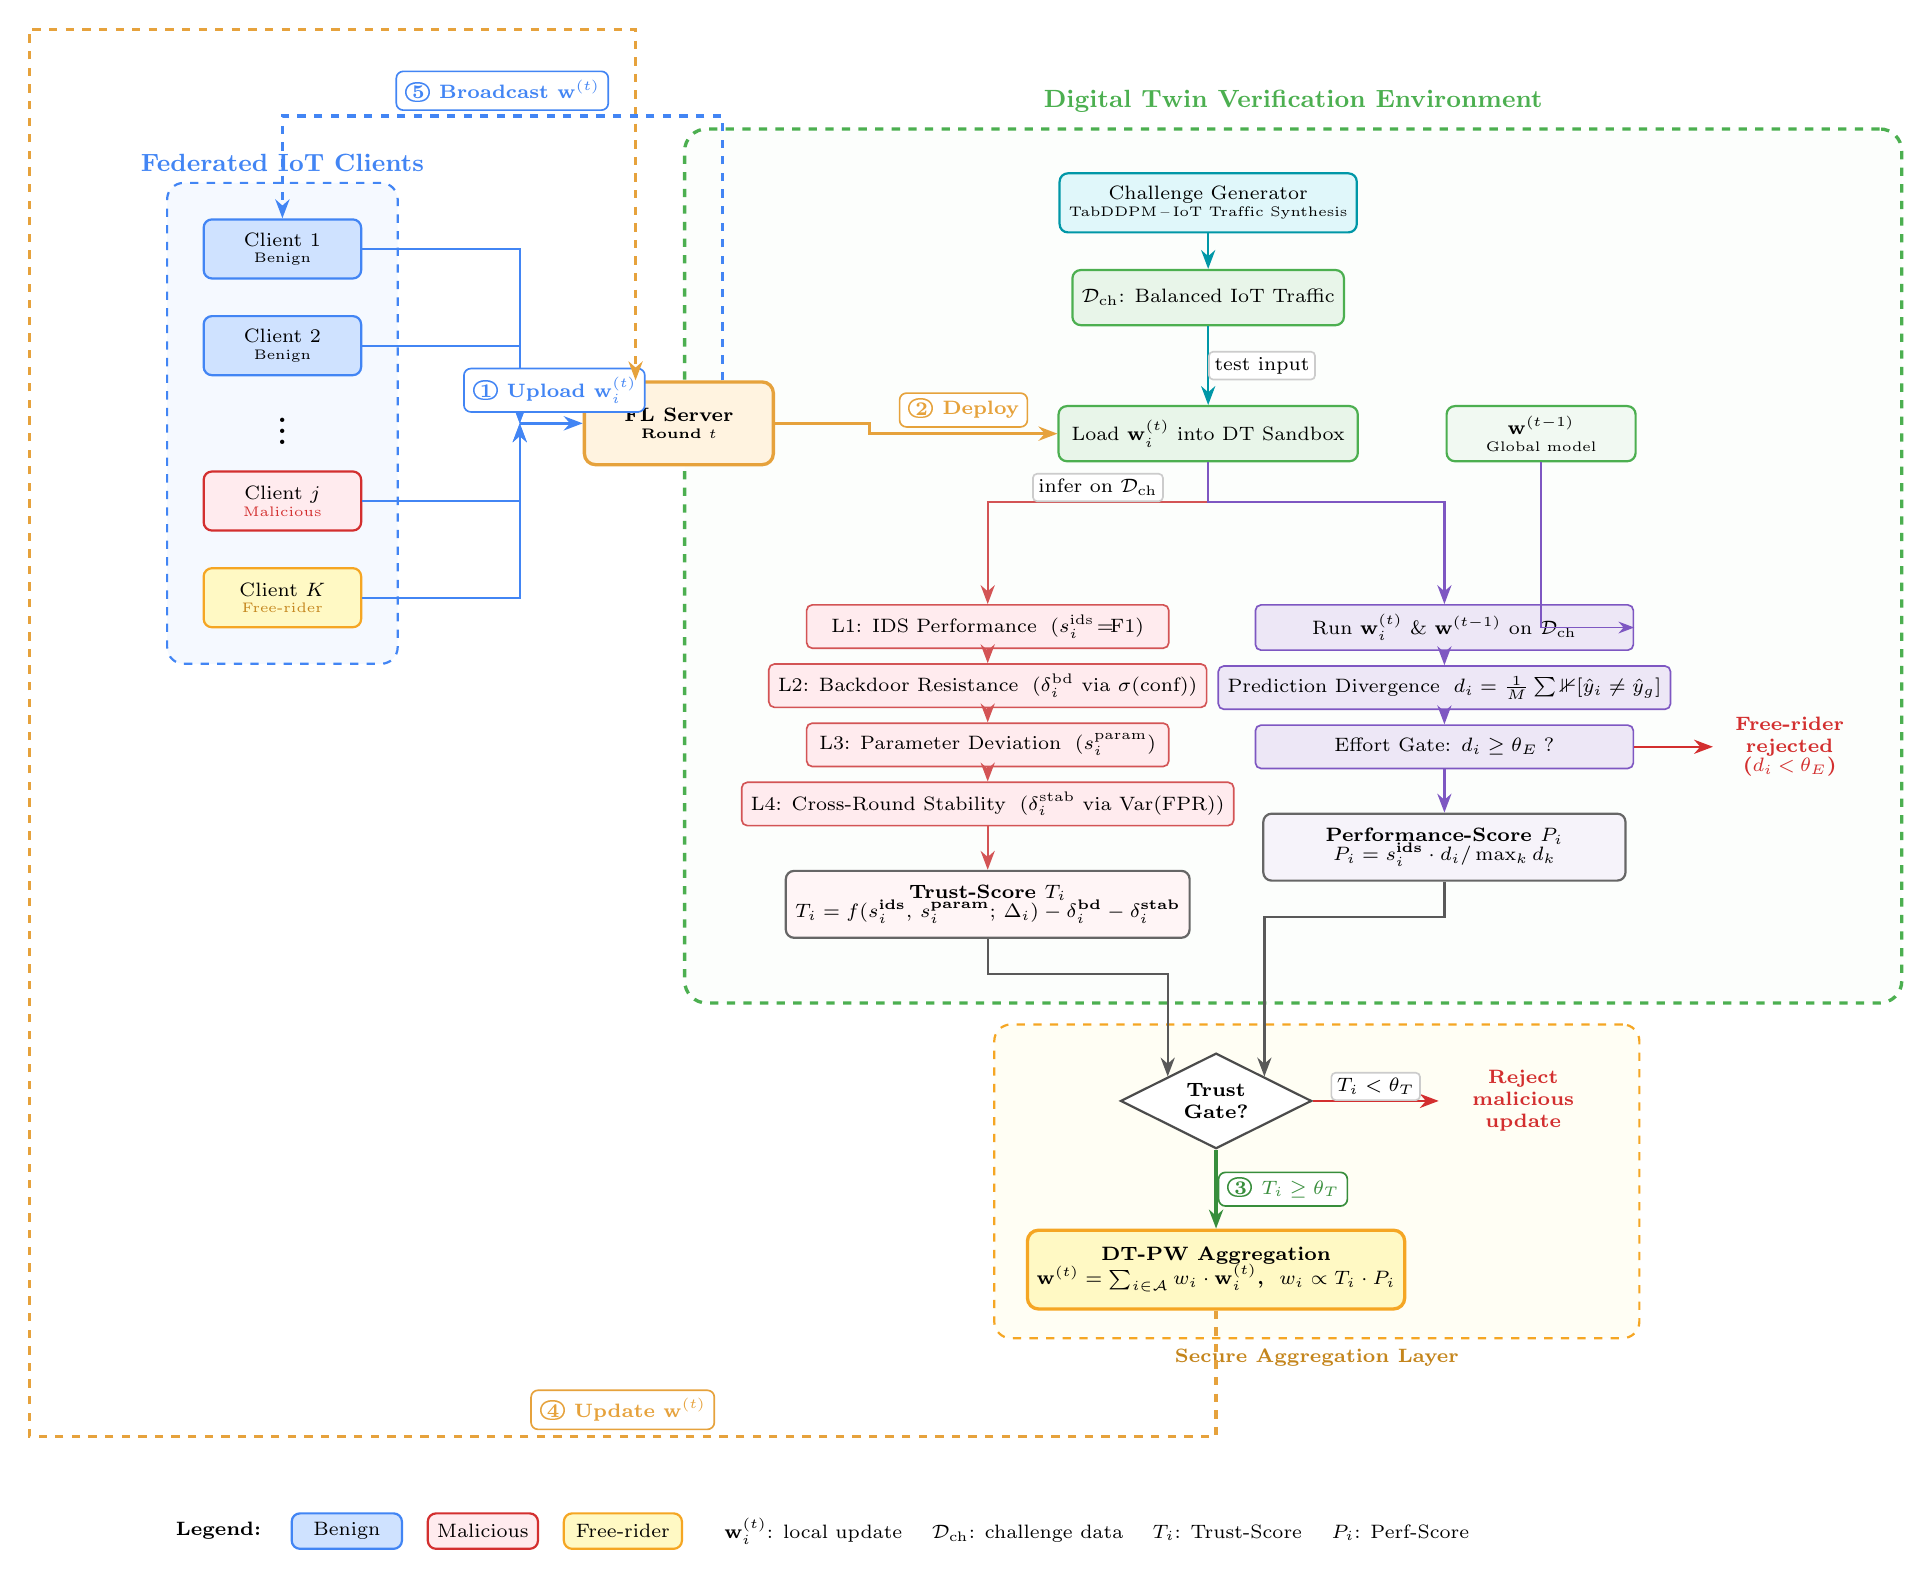
\begin{tikzpicture}[node distance=0.6cm and 0.9cm]

% ====================================================================
%  COLUMN 1 — Federated IoT Clients (far left)
% ====================================================================
\node[clientbox] (c1) {Client 1\\[-2pt]{\tiny Benign}};
\node[clientbox, below=0.45cm of c1] (c2) {Client 2\\[-2pt]{\tiny Benign}};
\node[font=\bfseries, below=0.20cm of c2] (cdots) {$\vdots$};
\node[clientbox, below=0.20cm of cdots,
      draw=rejectred, fill=verifyfill] (cm) {Client $j$\\[-2pt]{\tiny\color{rejectred} Malicious}};
\node[clientbox, below=0.45cm of cm,
      draw=aggedge, fill=aggfill] (cf) {Client $K$\\[-2pt]{\tiny\color{aggedge!80!black} Free-rider}};

% ====================================================================
%  COLUMN 2 — FL Server
% ====================================================================
\node[serverbox, right=2.8cm of $(c2.east)!0.5!(cm.east)$] (srv)
    {FL Server\\[-2pt]{\tiny Round $t$}};

% Upload arrows: each client -> common bundle point -> server
\coordinate (upBundle) at ($(srv.west) + (-0.8, 0)$);
\foreach \c in {c1,c2,cm,cf}{
    \draw[arr=iotblue] (\c.east) -| (upBundle);
}
\draw[arr=iotblue, very thick] (upBundle) -- (srv.west);

% Upload label: place on the bundle→srv segment, slightly above (in the gap
% between the client column and the server, away from any client box)
\node[steplbl=iotblue, text=iotblue]
    at ($(upBundle)!0.55!(srv.west) + (0, 0.42)$)
    {\cmark{1}\;Upload $\mathbf{w}_i^{(t)}$};

% ====================================================================
%  COLUMN 3 — DT Verification Environment
% ====================================================================

\node[genbox, right=3.6cm of srv, yshift=2.8cm] (gen)
    {Challenge Generator\\[-2pt]{\tiny TabDDPM\,--\,IoT Traffic Synthesis}};

\node[dtnode, below=0.45cm of gen] (dch)
    {$\mathcal{D}_{\text{ch}}$: Balanced IoT Traffic};

\node[dtnode, below=1.0cm of dch, minimum width=3.8cm] (deploy)
    {Load $\mathbf{w}_i^{(t)}$ into DT Sandbox};

% Server -> Deploy (Step 2) explicit polyline
\coordinate (depElbow) at ($(srv.east) + (1.2, 0)$);
\coordinate (depElbow2) at (depElbow |- deploy.west);
\draw[arr=serveredge, very thick]
    (srv.east) -- (depElbow) -- (depElbow2) -- (deploy.west);
\node[steplbl=serveredge, text=serveredge]
    at ($(depElbow2)!0.5!(deploy.west) + (0, 0.30)$)
    {\cmark{2}\;Deploy};

% Gen -> D_ch -> Deploy
\draw[arr=genedge] (gen) -- (dch);
\draw[arr=genedge] (dch) -- node[lbl, right] {test input} (deploy);

% Global model reference
\node[dtnode, right=1.1cm of deploy, minimum width=2.4cm,
      fill=dtfill!60] (gref)
    {$\mathbf{w}^{(t-1)}$\\[-2pt]{\tiny Global model}};

% ====================================================================
%  ROW 4 — Two parallel branches
% ====================================================================

% LEFT BRANCH: Four-Layer Pipeline
\node[vnode, below=1.8cm of deploy, xshift=-2.8cm] (v1)
    {L1: IDS Performance \;($s_i^{\text{ids}}\!=\!$F1)};
\node[vnode, below=0.18cm of v1] (v2)
    {L2: Backdoor Resistance \;($\delta_i^{\text{bd}}$ via $\sigma(\text{conf})$)};
\node[vnode, below=0.18cm of v2] (v3)
    {L3: Parameter Deviation \;($s_i^{\text{param}}$)};
\node[vnode, below=0.18cm of v3] (v4)
    {L4: Cross-Round Stability \;($\delta_i^{\text{stab}}$ via Var(FPR))};

\node[scorebox, below=0.55cm of v4, fill=verifyfill!50] (tscore)
    {Trust-Score $T_i$\\[-1pt]{\scriptsize $T_i = f(s_i^{\text{ids}},\, s_i^{\text{param}};\, \Delta_i) - \delta_i^{\text{bd}} - \delta_i^{\text{stab}}$}};

% Deploy -> V1 (left branch entry)
\coordinate (leftFork)  at ($(deploy.south) + (0,-0.5)$);
\coordinate (leftFork2) at (v1.north |- leftFork);
\draw[arr=verifyedge] (deploy.south) -- (leftFork) -- (leftFork2) -- (v1.north);
\node[lbl] at ($(leftFork)!0.5!(leftFork2) + (0, 0.18)$) {infer on $\mathcal{D}_{\text{ch}}$};

\draw[arr=verifyedge] (v1) -- (v2);
\draw[arr=verifyedge] (v2) -- (v3);
\draw[arr=verifyedge] (v3) -- (v4);
\draw[arr=verifyedge] (v4) -- (tscore);

% RIGHT BRANCH: DT-PW Scoring
\node[pwnode, below=1.8cm of deploy, xshift=3.0cm] (pw1)
    {Run $\mathbf{w}_i^{(t)}$ \& $\mathbf{w}^{(t-1)}$ on $\mathcal{D}_{\text{ch}}$};
\node[pwnode, below=0.18cm of pw1] (pw2)
    {Prediction Divergence \;$d_i = \frac{1}{M}\sum \mathbb{1}[\hat{y}_i \neq \hat{y}_g]$};
\node[pwnode, below=0.18cm of pw2] (pw3)
    {Effort Gate: $d_i \geq \theta_E$\;?};
\node[scorebox, below=0.55cm of pw3, fill=dtpwfill!50] (pscore)
    {Performance-Score $P_i$\\[-1pt]{\scriptsize $P_i = s_i^{\text{ids}} \cdot d_i / \max_k d_k$}};

% Deploy -> PW1 (right branch entry)
\coordinate (rightFork2) at (pw1.north |- leftFork);
\draw[arr=dtpwedge] (deploy.south) -- (leftFork) -- (rightFork2) -- (pw1.north);

% Global -> PW1
\draw[thinarr=dtpwedge] (gref.south) |- (pw1.east);

\draw[arr=dtpwedge] (pw1) -- (pw2);
\draw[arr=dtpwedge] (pw2) -- (pw3);
\draw[arr=dtpwedge] (pw3) -- (pscore);

% Free-rider rejected
\node[font=\scriptsize\color{rejectred}\bfseries,
      right=1.0cm of pw3, text width=1.7cm, align=center] (frlabel)
    {Free-rider\\rejected\\[-1pt]{\scriptsize ($d_i\!<\!\theta_E$)}};
\draw[arr=rejectred] (pw3.east) -- (frlabel.west);

% ====================================================================
%  BOTTOM — Decision Gate + Aggregation
% ====================================================================
\node[gatediamond, below=1.8cm of $(tscore.south)!0.5!(pscore.south)$] (gate)
    {Trust\\Gate?};

% Both scores -> Gate
\coordinate (tDown) at ($(tscore.south) + (0,-0.45)$);
\coordinate (pDown) at ($(pscore.south) + (0,-0.45)$);
\draw[arr] (tscore.south) -- (tDown) -| (gate.north west);
\draw[arr] (pscore.south) -- (pDown) -| (gate.north east);

% Reject path
\node[font=\scriptsize\color{rejectred}\bfseries,
      right=1.6cm of gate, text width=1.9cm, align=center] (rej)
    {Reject\\malicious update};
\draw[arr=rejectred] (gate.east) -- node[lbl, above] {$T_i < \theta_T$} (rej.west);

% Accept path -> Aggregation
\node[aggbox, below=1.0cm of gate] (agg)
    {DT-PW Aggregation\\[-1pt]{\scriptsize $\mathbf{w}^{(t)} = \sum_{i \in \mathcal{A}} w_i \cdot \mathbf{w}_i^{(t)}$,\; $w_i \propto T_i \cdot P_i$}};
\draw[arr=acceptgreen, very thick] (gate.south) -- (agg.north);
\node[steplbl=acceptgreen, text=acceptgreen]
    at ($(gate.south)!0.5!(agg.north) + (0.85, 0)$)
    {\cmark{3}\;$T_i \geq \theta_T$};

% ====================================================================
%  FEEDBACK LOOP — Update + Broadcast (clean "bus channel" routing)
% ====================================================================
% Reserve dedicated routing channels well outside every node so that
% feedback arrows never overlap clients, server top, or the client-group
% header label. Three channels:
%   chBot   : far below the diagram (below Aggregation)
%   chLeft  : far left of every client
%   chTopU  : above the client-group label  (Update bus)
%   chTopB  : above the client-group label, lower than chTopU (Broadcast bus)
\coordinate (chBot)  at ($(agg.south) + (0,-1.6)$);
\coordinate (chLeft) at ($(c1.west)   + (-2.2, 0)$);
\coordinate (chTopU) at ($(c1.north)  + (0,+2.4)$);
\coordinate (chTopB) at ($(c1.north)  + (0,+1.3)$);

% Split the server's top edge into two distinct anchors so Update (entering)
% and Broadcast (leaving) never share the same point.
\coordinate (srvNL) at ($(srv.north) + (-0.55, 0)$);
\coordinate (srvNR) at ($(srv.north) + (+0.55, 0)$);

% (4) Update: agg → bottom bus → left bus → top bus → into srvNL
\coordinate (u1) at (agg.south |- chBot);
\coordinate (u2) at (chLeft    |- chBot);
\coordinate (u3) at (chLeft    |- chTopU);
\coordinate (u4) at (srvNL     |- chTopU);
\draw[darr=serveredge, very thick]
    (agg.south) -- (u1) -- (u2) -- (u3) -- (u4) -- (srvNL);
% Place the label on the long bottom horizontal segment (clear empty zone)
\node[steplbl=serveredge, text=serveredge]
    at ($(u1)!0.5!(u2) + (0, 0.34)$)
    {\cmark{4}\;Update $\mathbf{w}^{(t)}$};

% (5) Broadcast: srvNR → up to lower top bus → left to above c1 → down to c1
\coordinate (b1) at (srvNR    |- chTopB);
\coordinate (b2) at (c1.north |- chTopB);
\draw[darr=iotblue, very thick]
    (srvNR) -- (b1) -- (b2) -- (c1.north);
% Place the label on the horizontal segment, well above the client-group label
\node[steplbl=iotblue, text=iotblue]
    at ($(b1)!0.5!(b2) + (0, 0.32)$)
    {\cmark{5}\;Broadcast $\mathbf{w}^{(t)}$};

% ====================================================================
%  BACKGROUND GROUPS
% ====================================================================
\begin{scope}[on background layer]
    \node[draw=iotblue, thick, dashed, rounded corners=6pt,
          fill=clientfill!20,
          fit=(c1)(cf),
          inner xsep=0.45cm, inner ysep=0.45cm,
          label={[font=\small\bfseries\color{iotblue}]above:Federated IoT Clients}] (clientgrp) {};

    \node[draw=verifyedge!70, thick, dotted, rounded corners=4pt,
          fill=verifyfill!20,
          fit=(v1)(v4)(tscore),
          inner xsep=0.25cm, inner ysep=0.25cm,
          label={[font=\scriptsize\bfseries\color{verifyedge}]above:Four-Layer Pipeline}] (pipegrp) {};

    \node[draw=dtpwedge!70, thick, dotted, rounded corners=4pt,
          fill=dtpwfill!20,
          fit=(pw1)(pw3)(pscore),
          inner xsep=0.25cm, inner ysep=0.25cm,
          label={[font=\scriptsize\bfseries\color{dtpwedge}]above:DT-PW Scoring}] (pwgrp) {};

    \node[draw=dtedge, very thick, dashed, rounded corners=8pt,
          fill=dtfill!12,
          fit=(gen)(dch)(deploy)(gref)(pipegrp)(pwgrp)(frlabel),
          inner xsep=0.45cm, inner ysep=0.55cm,
          label={[font=\small\bfseries\color{dtedge}, yshift=2pt]above:Digital Twin Verification Environment}] (dtgrp) {};

    \node[draw=aggedge, thick, dashed, rounded corners=6pt,
          fill=aggfill!18,
          fit=(gate)(agg)(rej),
          inner xsep=0.40cm, inner ysep=0.35cm,
          label={[font=\scriptsize\bfseries\color{aggedge!80!black}]below:Secure Aggregation Layer}] (agggrp) {};
\end{scope}

% ====================================================================
%  LEGEND (bottom, below the update arrow)
% ====================================================================
\path let \p1 = (clientgrp.west), \p2 = (u1) in
      coordinate (legAnchor) at (\x1, {\y2 - 1.2cm});

\node[anchor=west, font=\scriptsize\bfseries] (legtitle) at (legAnchor) {Legend:};
\node[clientbox, minimum width=1.4cm, minimum height=0.45cm,
      right=0.25cm of legtitle.east, anchor=west] (legben) {\scriptsize Benign};
\node[clientbox, minimum width=1.4cm, minimum height=0.45cm,
      fill=verifyfill, draw=rejectred,
      right=0.30cm of legben.east, anchor=west] (legmal) {\scriptsize Malicious};
\node[clientbox, minimum width=1.5cm, minimum height=0.45cm,
      fill=aggfill, draw=aggedge,
      right=0.30cm of legmal.east, anchor=west] (legfr) {\scriptsize Free-rider};
\node[anchor=west, font=\scriptsize, right=0.40cm of legfr.east, align=left]
    {$\mathbf{w}_i^{(t)}$: local update \quad
     $\mathcal{D}_{\text{ch}}$: challenge data \quad
     $T_i$: Trust-Score \quad
     $P_i$: Perf-Score};

\end{tikzpicture}
\end{document}




